\begin{figure}[!ht]
\centering
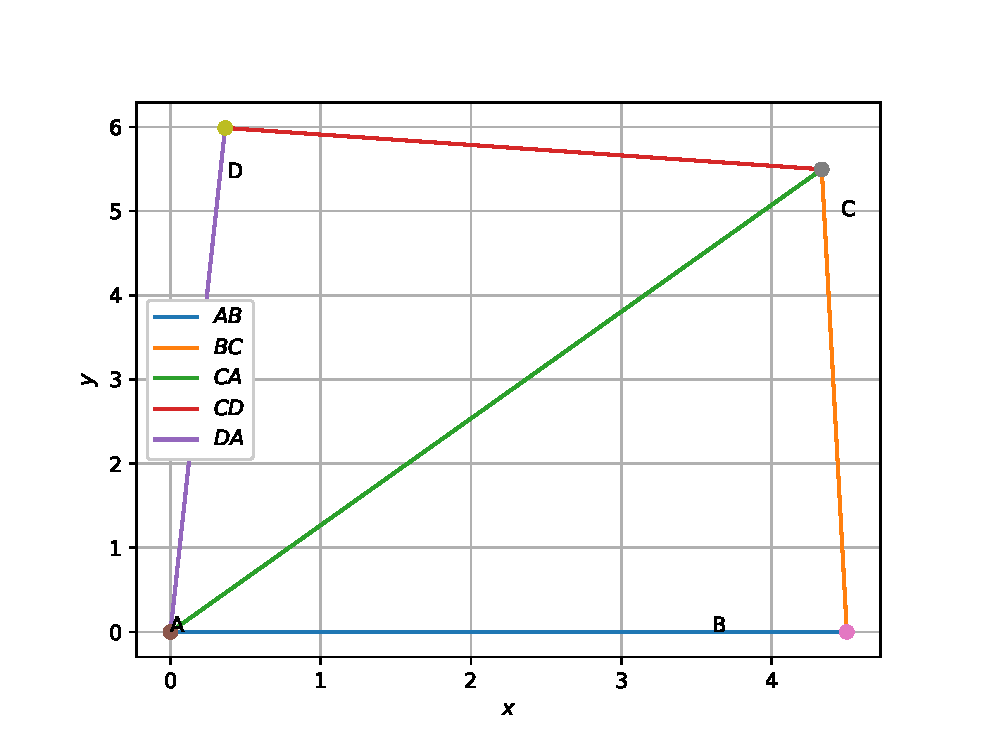
\includegraphics[width= \columnwidth]{./solutions/7/figs/quad/quad.eps}
\caption{Square ABCD}
\label{fig:2.2.7}
\end{figure}
See Fig. \ref{fig:2.2.7}

\begin{enumerate}
\item From inspection we see that the opposite vertices forms a diagonal which is parallel to x-axis. Then the diagonal formed by other two vertices is parallel to y-axis(i.e. their x coordinates are equal). Let $\vec{A}= \myvec{-1\\2}$  and $\vec{C}=\myvec{3\\2}$. 

\item In a square each interior angle is 90\degree and all sides are equal. Diagonals bisect each other at 90\degree.
Let $\vec{B}$ and $\vec{D}$ be other two vertices. 

\item If $\vec{x}$ is a vector then the given equations,
\begin{align}
\brak{\vec{x}-\vec{A}}^T\brak{\vec{x}-\vec{C}} &= 0 
\label{eq:eqn1}
\end{align}
\begin{align}
\norm{\vec{x}-\vec{A}} &= \norm{\vec{x}-\vec{C}}
\label{eq:eqn2}
\end{align}
are satisfied by $\vec{B}$ and $\vec{D}$. The \eqref{eq:eqn1} shows that the adjacent sides are perpendicular and \eqref{eq:eqn2} shows that length of the sides of the square are equal. On solving for $\vec{x}$, we get the value of $\vec{B}$ and $\vec{D}$. \\
Let $\vec{x}$ = $\myvec{x\\y}$, then from \eqref{eq:eqn1} 
\begin{align}
\myvec{x+1\\y-2}^T\myvec{x-3\\y-2} &= 0
\end{align}
\begin{align}
x^2 - 2x +1 +y^2 - 4y &= 0
\label{eq:eqn3}
\end{align}
From \eqref{eq:eqn2}
\begin{align}
\norm{\myvec{x+1\\y-2}}&=\norm{\myvec{x-3\\y-2}}
\end{align}
On solving we will get x= 1. Substiuting in \eqref{eq:eqn3}, we get y = 0,1.
Thus 
\begin{align}
\vec{B}&= \myvec{1\\0} \\
\vec{D}&= \myvec{1\\4}
\end{align} 
\item The python code for the figure can be downloaded from
\begin{lstlisting}
solutions/7/codes/quad/quad.py
\end{lstlisting}
\end{enumerate}  
